\documentclass[11pt, oneside]{article} 
\usepackage{geometry}
\geometry{letterpaper} 
\usepackage{graphicx}
	
\usepackage{amssymb}
\usepackage{amsmath}
\usepackage{parskip}
\usepackage{color}
\usepackage{hyperref}

\graphicspath{{/Users/telliott_admin/Tex/png/}}
% \begin{center} 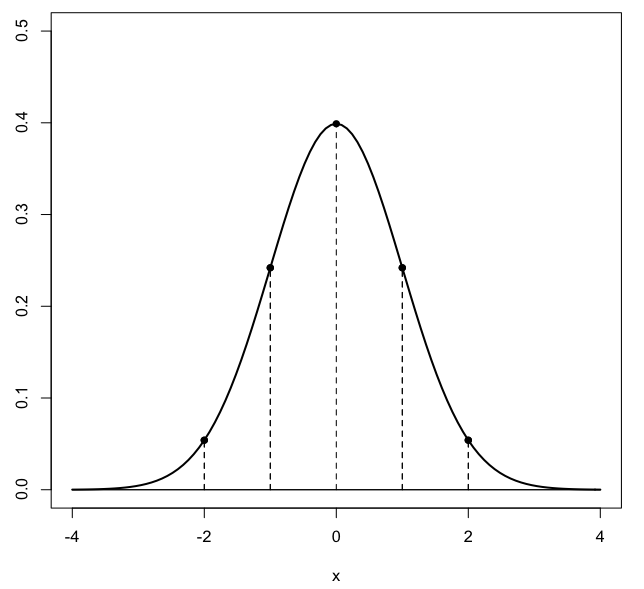
\includegraphics [scale=0.4] {gauss3.png} \end{center}

\title{Basic geometry and congruence of triangles}
\date{}

\begin{document}
\maketitle
\Large

\subsection*{Thales}
I'm a big fan of William Dunham's books --- three of them are listed in the References.  He talks about the history of mathematics in Greece, starting with Thales, who was from a Greek town called Miletus on the coast of Asia Minor (modern Turkey).  Although none of his writing survive, it is believed that Thales proved several early theorems including 

$\circ$  The vertical angles formed by two straight lines crossing, are equal.
\begin{center} 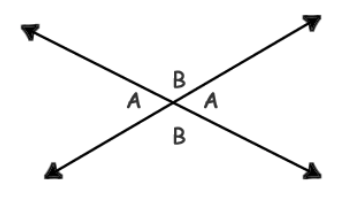
\includegraphics [scale=0.4] {vertical_angles.png} \end{center}
This theorem depends on a property of straight lines (that $A + B = 180$ degrees), and that "equals added to equals are equal."

$\circ$  The angle sum of a triangle equals two right angles.
\begin{center} 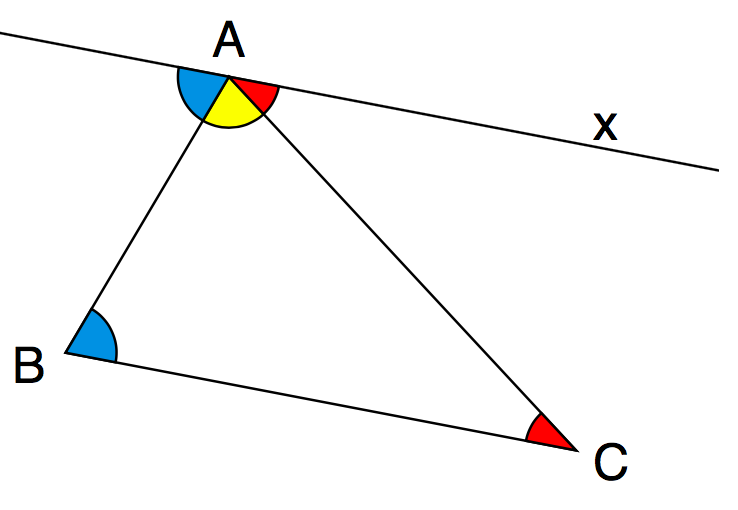
\includegraphics [scale=0.3] {triangle_sum_angles.png} \end{center}

This one depends on a theorem about alternate interior angles.

In the figure below, $A = D$ and $B = C$:
\begin{center} 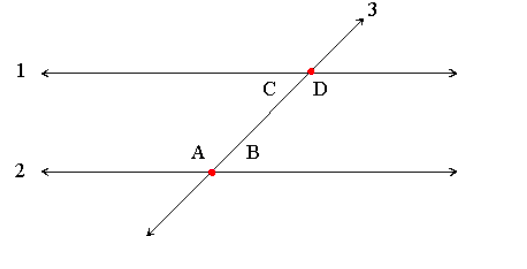
\includegraphics [scale=0.5] {alternate_interior_angles.png} \end{center}
which in turn depends on a property of parallel lines, that $A + C = 180$ degrees.  This is the famous parallel postulate:

\url{https://en.wikipedia.org/wiki/Parallel_postulate}

\subsection*{congruence and similarity of triangles}

$\circ$  Two triangles are congruent if they have the same three side lengths.  This is often abbreviated SSS (side-side-side).

Note that this definition means that the mirror image of a triangle is congruent to it.  The three triangles shown below are all congruent, even though the third is the mirror image of the first two.

\begin{center} 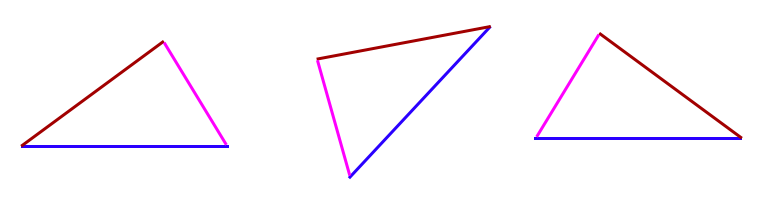
\includegraphics [scale=0.4] {congruent.png} \end{center}

$\circ$  Two triangles are similar if they have the same three angles.  Similar triangles are only congruent if they also have the same three sides.  The triangles shown below are similar.

\begin{center} 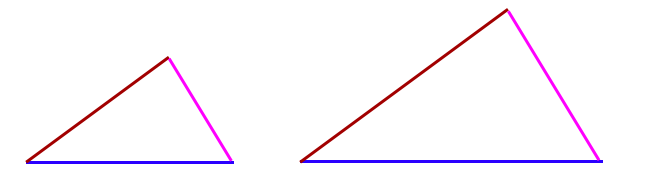
\includegraphics [scale=0.4] {similar.png} \end{center}

Given any triangle, draw a line parallel to one side, which also joins the other two sides.  The new triangle is similar to the given triangle.  Similarity means that all the angles are equal.  This is easily proved using the theorem on alternate interior angles.

\begin{center} 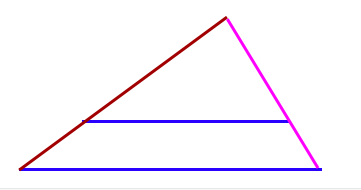
\includegraphics [scale=0.4] {parallel_line.png} \end{center}

In addition to SSS (side-side-side), there are other conditions that lead to congruence of two triangles when they are satisfied, namely

$\circ$  SAS (side-angle-side)

$\circ$  ASA (angle-side-angle)

$\circ$  AAS (angle-angle-side)

\subsection*{constructions}

The way I think about these conditions is to imagine trying to construct a triangle from the given information.  Suppose we know ASA.  The situation is thus:

\begin{center} 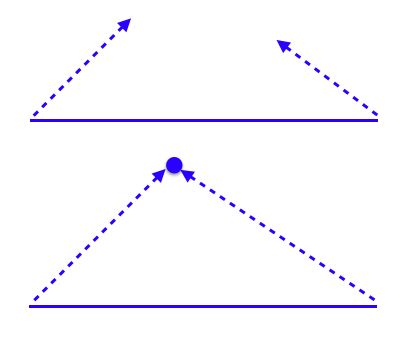
\includegraphics [scale=0.4] {ASA.png} \end{center}
 
Plot the known side and start two other sides from the ends of that side containing the known angles.  They must cross at a unique point.  

Or... actually, if we start the two lines pointing below the horizontal, there is another solution, the mirror image, which is also congruent, as discussed above.
 
Alternatively, knowing two angles means we also know the third, because they must add to 180 degrees.  For this reason, ASA and AAS, imply that we have exactly the same information, because we know all three angles and we also know which angles flank the known side.
 
Now consider a whole family of similar triangles.  Only one of those triangles has a side of a given length flanked by the two given angles.

For a right-triangle, if the hypotenuse and one leg are equal, the two triangles are congruent.

\begin{center} 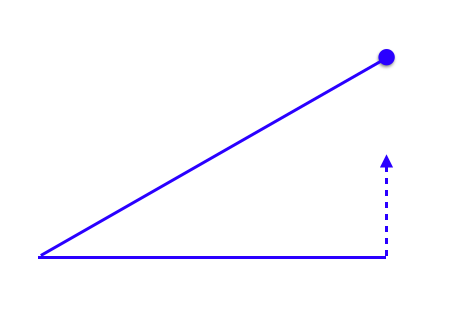
\includegraphics [scale=0.4] {hyp_side_congruent.png} \end{center}

In the figure, imagine the hypotenuse swinging on the hinge of its vertex with the horizontal base.  There is only one angle where it will terminate on the vertical side with the correct length.  This determines the length of the third side.
 
\subsection*{more theorems from Thales}

$\circ$  The base angles of an isosceles triangle are equal.

\begin{center} 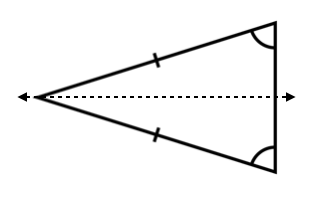
\includegraphics [scale=0.6] {isosceles.png} \end{center}
My favorite proof of the this one is from symmetry.  Draw a line from the vertex between the two equal sides to the midpoint of the base opposite.  If you turn the triangle over along this axis, we obtain the same triangle back again.  Alternatively, just say "side-side-side."

$\circ$  Any angle inscribed in a semicircle is a right angle.

This diagram really gives the whole proof away.
\begin{center} 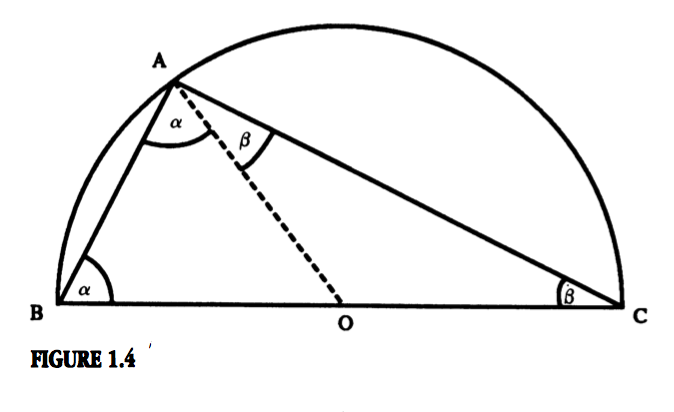
\includegraphics [scale=0.4] {right_angle2.png} \end{center}

\subsection*{pentagon} 

Let's practice these concepts by analyzing the regular pentagon, a polygon with five sides of equal length.  Draw a pentagon and all five of its internal chords.
\begin{center} 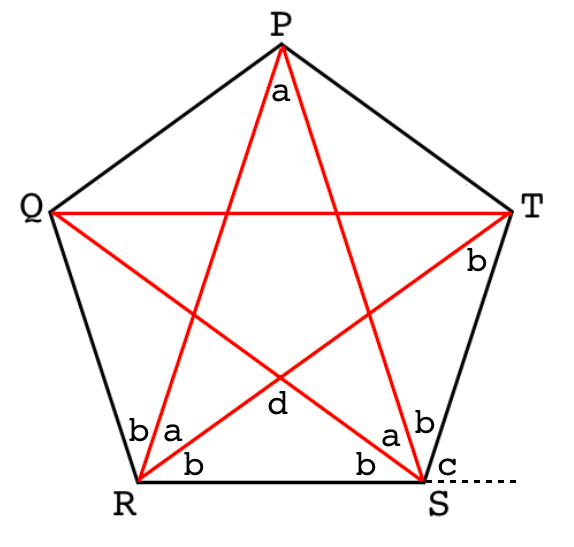
\includegraphics [scale=0.35] {pent_chords.png} \end{center}

By rotational symmetry, the total angle at each vertex is the same.  The supplementary angle to this angle is $c$.

One way to get the measure of the angles is to imagine that we walk along the base $RS$ and then make a left-turn at $S$, to face $T$.  The angle through which we turn is $c$.  In going around the whole perimeter to return to R (and face horizontally again) we turn 5 times.  Hence $5c = 2 \pi$
or
\[ c = \frac{2}{5} \cdot \pi \]

Now, it will turn out that all the angles in the figure are some multiple of $\pi/5$.  For example, the vertex angle (call it $v$) is 
\[ v = \pi - c =  \frac{3}{5} \cdot \pi \]

Another way to obtain this result is to use the formula we will prove later (by induction) that
\[ (n-2) \cdot \pi = S \]
where is $S$ is the sum of the internal angles.  We obtain
\[ (5 - 2) \cdot \pi = 5 v \]
\[ v = \frac{3}{5} \cdot \pi \]

The angles labeled $a$ are all equal (as well as some equivalent angles that aren't labeled), by the rotational symmetry of the figure.  There are 5 such angles in total.  

By symmetry, all the angles labeled $b$ are also equal (some of these aren't labeled, as well).  

Consider the triangles $RST$ and $PRS$.  Adding angles, we have that 
\[ a + 4b = \pi = 3a + 2b \]
\[ 2b = 2a \]
\[ a = b \]

Since each vertex has two copies of $a$ and one of $b$
\[ v = 2a + b = 3a = \frac{3}{5} \cdot \pi \]
\[ a = b = \frac{1}{5} \cdot \pi \] 
\begin{center} 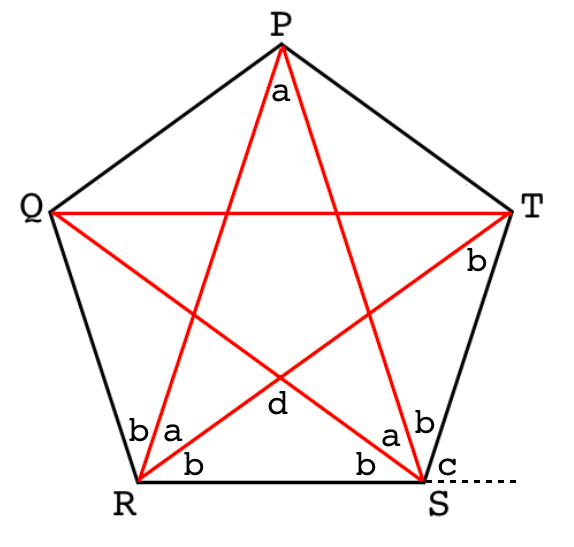
\includegraphics [scale=0.35] {pent_chords.png} \end{center}

The inner polygon is also a pentagon.  Since $2b + d = \pi$
\[ d =  \frac{3}{5} \cdot \pi \]
which is the same as vertex angle of the original pentagon.

By symmetry, all the angles of the inner pentagon are equal, so it is a regular pentagon.

Triangle $PRS$ is isosceles.  By symmetry, or by equal base angles $2a$, the triangle formed by $P$ plus the chord $QT$ is also isosceles.  So that triangle is similar to $PRS$ and therefore chord $QT$ is parallel to the base $RS$.

One can draw two types of isosceles triangles using the chords and sides of the pentagon.  One is short and fat, the other, tall and skinny.  The first type have base angles equal to $2/5 \cdot \pi$ and the second, base angles equal to $1/5 \cdot \pi$.  Here are three examples of tall and skinny:
\begin{center} 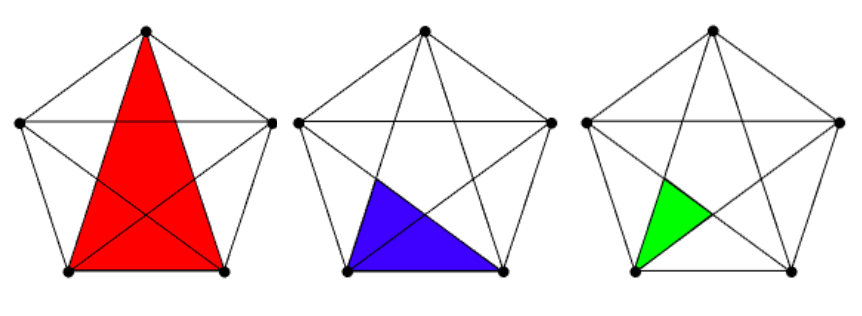
\includegraphics [scale=0.4] {three_triangles.png} \end{center}

The figure also contains regular parallelograms with base angles $a+b$ and $a + 2b$.  
 \begin{center} 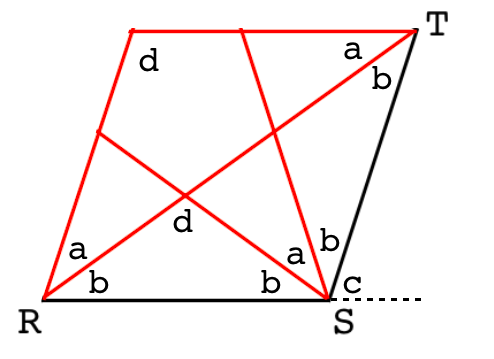
\includegraphics [scale=0.4] {pent_quad.png} \end{center}
 
In this figure, the diagonal $RT$ forms two congruent triangles (by ASA).  Therefore the sides formed by portions of chords of the pentagon are equal in length to the side of pentagon.  That is, all side lengths of the quadrilaterals are equal.

As a consequence, the portion of any chord that crosses over one other chord but does not reach all the way to the next vertex has the same length as a side.

If we take the side length of the original pentagon to be 1, then the length of the long side of the red triangle is $1$ plus some other value, call that $x$.  

But $x$ is also the length of the short side or base for the blue triangle.  We use the fact that red and blue are similar and form the ratio $\phi$ of the long side to the base (red on the left, blue on the right):
\[ \phi = \frac{1 + x}{1} = \frac{1}{x} \]
Rearrange:
\[ x^2 + x - 1 = 0 \]
\[ x = \frac{-1 \pm \sqrt{1 + 4}}{2} \]
Of course, $\phi$ is the golden ratio where we have taken the positive branch of the square root:
\[ \phi = 1 + x = \frac{1 + \sqrt{5}}{2} \]

\subsection*{analytic geometry}

It is assumed you've studied analytic geometry before.

It is difficult today to put ourselves in the places of those who tried to reason about mathematics through the ages.  For example, the Greeks lacked algebra, and although the Romans worked with numbers they lacked decimal notation.  The concept of $0$ came much later (from India), and even in the Middle Ages there was as yet no such thing as the equals sign $=$, which dates from 1557.

\url{https://en.wikipedia.org/wiki/Table_of_mathematical_symbols_by_introduction_date}

The invention of analytic geometry is often ascribed solely to Descartes, but Fermat also had a big role.  There are two fundamental ideas.
\begin{center} 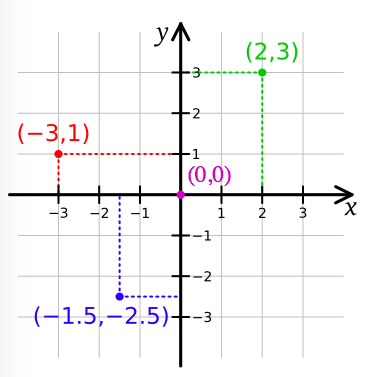
\includegraphics [scale=0.6] {coordinates.png} \end{center}

The first is to orient two number lines on a piece of paper, at right angles, and then consider pairs of numbers $(x,y)$) in the 2D plane.  Such pairs or tuples are called points.

The second idea is to plot all the points that satisfy some mathematic relationship between $x$ and $y$, for example the parabola $y=x^2$.  We sketch the graph of the curve, without actually trying to plot all of the individual points (of which there is an infinite number).

Here is a moderately complicated example we will see much later in the book.
\begin{center} 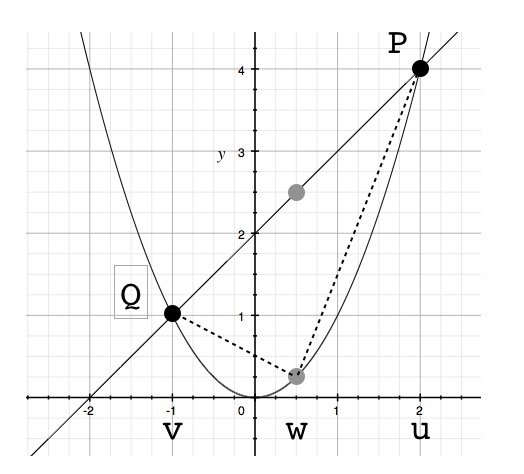
\includegraphics [scale=0.4] {para_tri2.png} \end{center}

It shows the two axes (horizontal and vertical lines with distances marked), and four points plotted plus a line, two line segments, and a parabola.  We can also "read" other points off the graph, such as the vertex of the parabola $(0,0)$, or the intersections of the line with the axes at $(-2,0)$ and $(0,2)$.

\end{document}